\documentclass[letterpaper, 10 pt, conference]{ieeeconf}  % Comment this line out
                                                          % if you need a4paper
%\documentclass[a4paper, 10pt, conference]{ieeeconf}      % Use this line for a4
                                                          % paper

\IEEEoverridecommandlockouts                              % This command is only
                                                          % needed if you want to
                                                          % use the \thanks command
\overrideIEEEmargins
% See the \addtolength command later in the file to balance the column lengths
% on the last page of the document

% Add additional packages here if required
\usepackage{color}
\definecolor{highlight}{rgb}{1,1,0.6}
\definecolor{link}{rgb}{0.5,0.0,0.0}
\definecolor{cite}{rgb}{0.0,0.0,0.6}
\definecolor{url} {rgb}{0.3,0.0,0.3}
\definecolor{grey}{rgb}{0.3,0.3,0.3}
\usepackage{siunitx}
\usepackage{adjustbox} % by awa
%***
\usepackage{listings}
\usepackage{url}
\usepackage{array, makecell} %

\usepackage[linesnumbered,ruled]{algorithm2e} % used for algorithms
\newcommand\mycommfont[1]{\footnotesize\ttfamily\textcolor{blue}{#1}}
\SetCommentSty{mycommfont}
%***
\usepackage{amsmath}
\usepackage{graphicx}
\usepackage{fancybox}
\usepackage{rotating} % to rotate the table
\usepackage{multirow} % used to merger columns in table
\usepackage{soul} % for highlighting text
\usepackage{relsize} % used in the \anote and \comment macros.
\usepackage{subfig} % used to put figure side by side
\usepackage{mathtools}
\DeclarePairedDelimiter{\ceil}{\lceil}{\rceil}

\newcommand{\quotes}[1]{``#1''} 
\makeatletter
\newcommand{\mathleft}{\@fleqntrue\@mathmargin15pt}
\newcommand{\mathcenter}{\@fleqnfalse}
\makeatother

\newcommand{\mynote}[1]{{\leavevmode\smaller\itshape\color{red}\{#1\}}}
\sethlcolor{highlight}
\newcommand{\mycomment}[2]{\hl{#1} {{\leavevmode\smaller\color{red}\itshape\{#2\}}}}

\newcommand{\anote}[1]{{\leavevmode\smaller\itshape\color{red}\{#1\}}}

\newcommand{\topic}{\ensuremath{\mathit{T}}}
\newcommand{\bs}{\ensuremath{\mathit{BS}}}
\newcommand{\ti}{\ensuremath{\mathit{TI}}}
\newcommand{\mr}{\ensuremath{\mathit{MR}}}
\newcommand{\up}{\ensuremath{\mathit{UP}}}
\newcommand{\doff}{\ensuremath{\mathit{DO}}}
\newcommand{\tati}{\ensuremath{\mathit{TATI}}}
\newcommand{\etm}{\ensuremath{\mathit{ETM}}}
\newcommand{\tp}{\ensuremath{\mathit{TP}}}
\newcommand{\bn}{\ensuremath{\mathit{BN}}}
\newcommand{\smartc}{\ensuremath{\mathit{SC}}}
\newcommand{\rt}{\ensuremath{\mathit{RT}}}
\newcommand{\bt}{\ensuremath{\mathit{BT}}}
\newcommand{\rtEst}{\ensuremath{\widehat{\mathit{RT}}}}

\newcommand{\crep}{\ensuremath{C_{\mathit{rep}} }}

\newcommand{\gt}{\ensuremath{\mathit{GT}}}
\newcommand{\rc}{\ensuremath{\mathit{RC}}}   % receipt cost
\newcommand{\gup}{\ensuremath{\mathit{GUP}}}
%
% The following packages can be found on http:\\www.ctan.org
\usepackage{graphics} % for pdf, bitmapped graphics files
%\usepackage{epsfig} % for postscript graphics files
%\usepackage{mathptmx} % assumes new font selection scheme installed
%\usepackage{times} % assumes new font selection scheme installed
\usepackage{amsmath} % assumes amsmath package installed
\usepackage{amssymb}  % assumes amsmath package installed

\title{\LARGE \bf
Decentralized Marketplace for Brokered IoT Data Trades using Blockchain
}

%\author{ \parbox{3 in}{\centering Huibert Kwakernaak*
%         \thanks{*Use the $\backslash$thanks command to put information here}\\
%         Faculty of Electrical Engineering, Mathematics and Computer Science\\
%         University of Twente\\
%         7500 AE Enschede, The Netherlands\\
%         {\tt\small h.kwakernaak@autsubmit.com}}
%         \hspace*{ 0.5 in}
%         \parbox{3 in}{ \centering Pradeep Misra**
%         \thanks{**The footnote marks may be inserted manually}\\
%        Department of Electrical Engineering \\
%         Wright State University\\
%         Dayton, OH 45435, USA\\
%         {\tt\small pmisra@cs.wright.edu}}
%}

\author{Shaimaa Bajoudah$^{1,2}$, Changyu Dong$^{1}$ and Paolo Missier$^{1}$% <-this % stops a space
% \thanks{*This work was not supported by any organization}% <-this % stops a space
\thanks{$^{1}$School of Computing, Newcastle University, Newcastle Upon Tyne, The UK.
         Email: s.bajoudah1@ncl.ac.uk, Changyu.Dong@ncl.ac.uk and Paolo.Missier@ncl.ac.uk}%
\thanks{$^{2}$College of Computer and Information Systems, Umm AlQura University, Makkah, KSA. Email: sbajoudah@uqu.edu.sa}%
}


\begin{document}


\maketitle
\thispagestyle{empty}
\pagestyle{empty}


%%%%%%%%%%%%%%%%%%%%%%%%%%%%%%%%%%%%%%%%%%%%%%%%%%%%%%%%%%%%%%%%%%%%%%%%%%%%%%%%
\begin{abstract}

As data marketplaces are becoming commonplace, it is also becoming clear that data streams generated from Internet of Things (IoT) devices hold value for potential third party consumers.
We envision a marketplace for IoT data streams that can unlock such potential value in a scalable way, by enabling any pairs of data providers and consumers to engage in data exchange transactions without any prior assumption of mutual trust.
We present a marketplace model and architecture to support trading of streaming data, from the advertising of data assets to the stipulation of legally binding trading agreements, to their fulfilment and payment settlement. Crucially, we show that by using blockchain technology and Smart Contracts in particular, we can offer participants a trade-off between the cost of transactional data exchange, and the risk of data loss when trading with untrusted third parties.
We experimentally assess such trade-offs on a testbed using Ethereum Smart Contracts.
%
%data are increasingly viewed as a new form of massively distributed and large scale digital assets, which are continuously generated by millions of connected devices. The real value of such assets can only be realized The IoT data that are generated from IoT devices has shown a new insight to do profitable business. Any IoT data owner industries or individuals can sell their data into a marketplaces and get some profits. This paper has introduced a decentralized marketplace for real-time IoT data streams with the use of the Blockchain technology. A producer publishes offers to what streams has, and a consumer request a trade based on the proposed offers. Then a data producer and data consumer has a trade agreement  TA for their trade recorded in the Blockchain and executed if the contractual obligation has been met. An honest consumer who send receipts with the exact amount of data received. It shows a direct proportion between a consumer honesty and trade's cost done in this marketplace. It has been evaluated that an honest consumer cost less than dishonest consumer to get involved in trades in this marketplace. 

\end{abstract}


%%%%%%%%%%%%%%%%%%%%%%%%%%%%%%%%%%%%%%%%%%%%%%%%%%%%%%%%%%%%%%%%%%%%%%%%%%%%%%%%
\section{INTRODUCTION}


\mynote{need to ACK our IOT paper and relate back to it}


\anote{minor: make sure links to sites etc are not part of biblio -- only use biblio for academic references.  put urls inline \url{blah} or as footnotes}

\anote{intro still requires major edits -- I will work on it}

The Internet of Things (IoT) is a dynamic global network for objects that are connecting together by the Internet such as sensors, actuators and Radio-frequency identification (RFIDs) to provide value-added services. Over the last decade, the IoT data has become one of the traceable assets in current ecosystem due to its beneficial aspects for their owners and their buyers. Data marketplaces \anote{for IoT data} have emerged which present a platform for data owners and buyers to negotiate and apply terms that both agreed to trade the needed data \cite{misura}.

Currently, there are many projects working as a marketplace for data trading. \mycomment{Some of them}{need references} are showing a shared economy with real-time IoT data which generated from IoT devices in many domains. \mycomment{Many of them}{need references} are offering various datasets to be sold for either individuals, government or industries for the aggregation and analysis purposes. These traditional marketplaces has been selling the datasets where the data are not updated or not time sensitive. Unlike the marketplaces for real-time data that are generated from IoT. It is a difficult task to  design marketplaces for IoT data due to its characteristics which make them different from traditional datasets. \cite{misura} has shown unique IoT data features. The undependability of IoT data owner is one of its uniqueness. There are variety of IoT owner who produce data from their owned devices and sell it. In addition, IoT data are gathered from real-time sensors such as temperature, humidity or car traffic is time sensitive. If these data has not been used at the time of its generation it would loose their value and no longer needed. And because of the IoT data is time sensitive, a data buyer would have a trade agreement to buy data in advance which is a challenging task. Buying data in advance needs a mechanism in the marketplace to decide if the payment would be paid before of after delivering the data. If it is before subscribing the data, that means we require a system to fulfill the trade agreement that data provide and data buyer have, enforce the contract obligations to be done and guarantee delivering data to the consumers.

Currently, it has sown many marketplaces that are tailored to deal with IoT data in either centralized or in decentralized infrastructure. Misura in \cite{misura} has introduced a centralized marketplace as a cloud application based on a queuing system. Each data provider registers their sensors into the application with all details and description of the data. On the other hand, data consumer query the system for their needs and then  they will be advised by the system to the appropriate data provider who provide their needs. 

On the other hand, Datum \cite{24} has introduced a decentralized marketplace based on the emerging technology Blockchain. It is an IoT data marketplace which is designed to trade a stored IoT data based on Ethereum Blockchain network. A data provider achieves the scalability by storing his structural data securely in such BigchainDB and IPFS.  It uses the smart contract and the DAT token to enable the data buyer to get access to these data. 

The vision of our model is to have a decentralized marketplace for real-time IoT data with the use of the distributed ledger (Blockchain). It consists of two layers; data layer for exchanging data in the brokerage platform and Blockchain layer for the negotiation and trades contracts.

The remainder of this paper is organized as follows. Section \ref{CentModel} shows the centralized model. Section \ref{Motivation&Contribution} and \ref{RelatedWork&Background} show the motivation of our model and the related works. Section \ref{MKModel} and section \ref{Arch} show the marketplace model and the system architecture. Section \ref{Impl&Evaluation} shows the implementation and the evaluation of  consumer cost in the marketplace and then it will be ended by the conclusion in section \ref{conclusion}.

\subsection{Centralized Brokered IoT Data Marketplace Architecture} \label{CentModel}

\begin{figure}
  \caption{Centralized Brokered IoT Data Marketplace Architecture}
  \label{fig:brokered-data-exchange}
  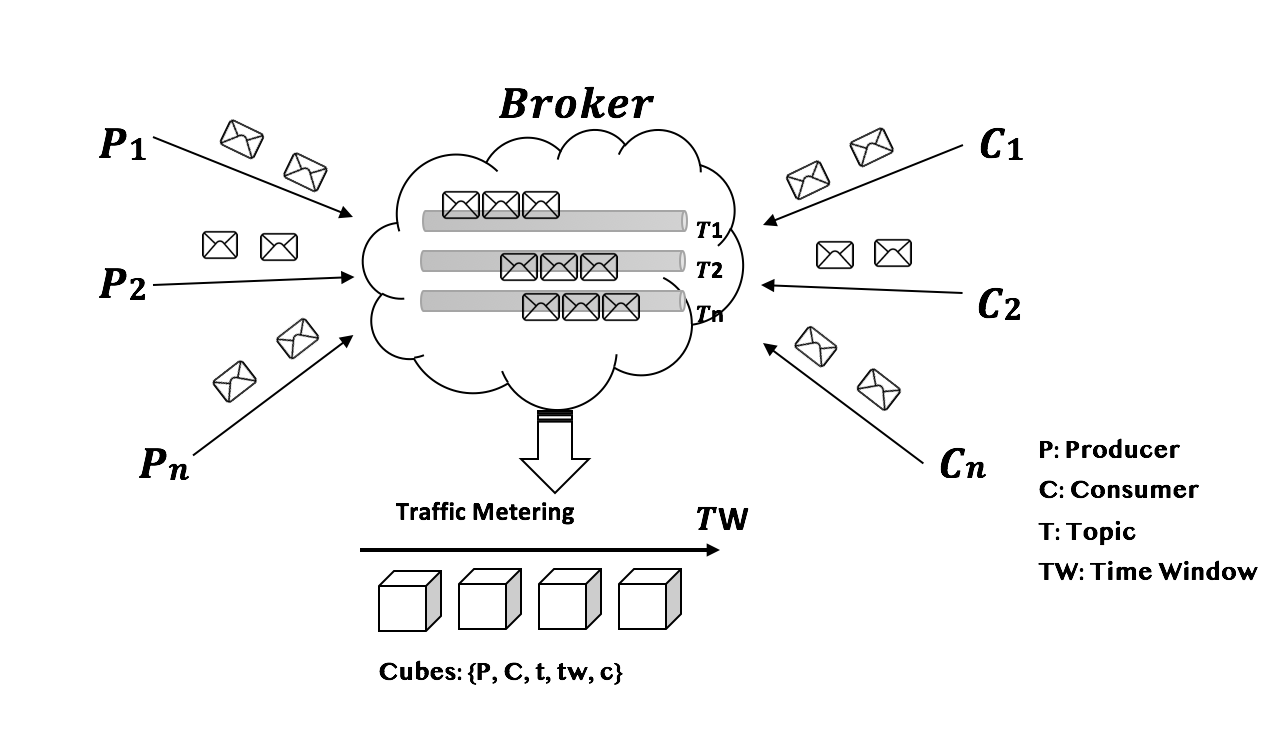
\includegraphics[scale=0.4]{Cent}
%   \centering

\end{figure}

Recent days, sharing the economy with IoT data has increased the demand for establishing IoT data marketplace. In brokered IoT data marketplace scenario as shown in Figure\ref{Cent} , data providers have to push their data through a centralized broker which then data consumers subscribe through predefined topics. A broker has the ability to count the number of messages published by a producer and subscribed by a consumer for all producers and consumers participated in the marketplace, which is dependable as a data source for the settlement process. The settlement process relies on the data metering from the broker and applies the settlement straightforward for both producer and consumer. 
	
In the above centralized reward data marketplace model, with the assumption of removing the trust from the broker, it could be a threat to alter or change some of data traffic metering between producers and consumers which would affect on the data authenticity, therefore the settlement process would be unsatisfied. This could be a vital factor in the marketplace sustainability especially with the absence of the trust and the lack of other secondary dependencies could be used to check the missed or altered metering data of the trade.
The centralized infrastructure, as well as the third party- intermediators for data exchange, is not a centralized trusted component. It has been watched by the researchers that the trust issue has limited sharing data and killed the enthusiasm to be part of unreliable marketplace. While some of the current platforms have strength their model by many security mechanisms such as access control and authentication privacy, they still depend on the third party \cite{12}.

\subsection{Motivation and Paper Contribution} \label{Motivation&Contribution}
%%%%%%%%%%%%%%%%%%%%%%%%%%%%%%

\anote{
-- what problem has not been solved: marketplace with (i) IoT streaming data and (ii) no mutual trust amongst participants. \\
-- approach: (i) smart contract act as broker. (ii) mechanisms to reduce risk on both sides in the absence of trust: (ii-a) protocol involving smart contract to record transactions, and (ii-b) reputation model to mitigate risk. The two are connected: the protocol allows data exchange to be tuned in a way that is a function of limited trust, acquired through the reputation model.
}


In our previous work\cite{Missier2017} we suggested that the next generation of marketplaces for IoT data  should meet four main requirements;Dynamicity,Access to individuals, Real-time streams as a marketplace assets and decentralization of trust with governance.

 The marketplace should be able to flexibly accept new participants (either individuals, institutions or business organizations), be resilient to leaving participants, and accommodate unanticipated business relationships amongst those participants. That means anyone who controls IoT devices and generate IoT data streams should be able to monetize it and use it as a tradeable assets in the marketplace.
 
Although the current traditional data marketplaces such as the Microsoft's Azure Data Market \cite{22} cater to batch static data with long ''shelf life'', our focus is on streams whose value is maximal when they are consumed ''live'' (as opposed to being stored and played back on demand).

Additionally, in contrast to existing proposals, e.g.\cite{Cao:2016:MMR:2926746.2883611}, we aim to define a marketplace that does not require a centralized trust component, such as a brokerage platform with trusted ownership, but relies instead on collective verification mechanisms, such as blockchain, to enforce its own governance rules.

In this paper we describe a Blockchain-based marketplace architecture that is designed to fulfill all of these requirements. It is a challenging task to have a public decentralized marketplace dealing with a live stream with no trusted component.

% In addition, a blockchain is not designed to record too much data, so it has to employ the advantages of the blockchain in the marketplace for trades' obligations fulfillment and data exchange monitoring in the brokerage platform with taking into account the blockchain limitation e.g. scalability.

% The emerging of the decentralized applications has emphasized the lack of reliance on the third party and killed the fact of trusting an individual node.  It shows a wide area for applications with no failure point due to decentralized infrastructure. 

 In our decentralized model, the settlement and the trade monitoring is done on the blockchain layer which means that we need a level of trust to accomplish theses trades successfully. The blockchain gives the opportunity to remove the third party that guarantee the trust in the centralized model , and instead distribute the trust and placed elsewhere, namely in public key cryptography and a ''consensus mechanism'' that allows us to determine the truth.

Real-time IoT data has minimal value when they are not used at the same time of its generation, so we need a model dealing immediately with the data. In addition, the blockchain was not emerged to store a huge amount of data and instead, it is created to store limited data immutably. 

With the core advantage of the second generation of the blockchain – smart contract – we propose each trade must have a digital contract called Trade Agreement TA. Each TA must be signed by both parties and once its obligations are met, it is executed automatically and all trades payments are done in Ethereum token (Ether).

% For this, unlike the IOTA project \cite{20}, there is no need to record all IoT data in the chain and only need to store the metadata and the trade details between a producer and a consumer as a trade agreement. With the core advantage of the second generation of the blockchain – smart contract – we propose each trade must have a digital contract called Trade Agreement TA. Each TA must be signed by both parties and once its obligations are met, it is executed automatically and all trades payments are done in Ethereum token (Ether).

\subsection{Background and Related Works} \label{RelatedWork&Background}

Literately, the blockchain technology is not a new concept in the computer community, it is just the result of the combination of three old concepts, peer-to-peer networks, public key cryptography and distributed consensus based on resolution random math challenges (Cryptographic hashing) \cite{2}. It can be defined as a fully-distributed, peer to peer network platform which can record immutable data, host applications \cite{2} and even transfer the ownership of digital assets which has a monetary value in the reality. Although it currently comes at a great computational cost, the characteristic of not relying on a trusted third party is held as their most important characteristic.

With the assumption of having a decentralized marketplace for IoT data leveraged by blockchain technology, we guarantee the trustworthy and transparency. The Immutability of transactions recorded in the blockchain is one of its strength and the key factor of providing a digital trustless environment to businesses. In the blockchain network, each transaction has been sent to the network is secure and transparent, thereby making the use of blockchain as a business infrastructure a good choice.

Recently, many of financial sectors take the benefits of the blockchain (security, immutability, transparency) and trying to dispense with the intermediation and it will change the shape of companies’ friction everywhere \cite{2}\cite{9}\cite{10}. In the scenario of brokered IoT data marketplace, it is no longer need to pay fees for settlement provider to do the settlement in an untrusted environment. Moving to the decentralization infrastructure using blockchain solves one of critical issues in the in distributed environment as each node has to have the same version and the last update of the records.

The second generation of blockchain has introduced the smart contract. Any party in a business can move their contractual obligations to the blockchain network by writing their agreements as the form of smart contract and deploy it to the network. A smart contract is a piece of code (written in special high-level languages for writing contracts in blockchain such as Solidity) which is used to govern transactions exchanges between network nodes. It has been becoming the substitution to traditionally written contracts because of its key elements: autonomy, automation, and decentralization\cite{8}.  

The monetization of the huge amount of IoT data generated from its devices is a challenging task when taking in consideration many issues related to automation and scalability. There are many marketplaces tailored to deal with IoT data in various infrastructure e.g. centralized and decentralized which nourish the IoT data ecosystems either from individuals or companies e.g. Datacup, Microsoft Azure, sale’s data.com and BDEX. These projects are maintained by a central authority which controls and manage the trade between data provider and data buyer. Big IoT Marketplace \cite{14} is one example. It is a European project to enable IoT Ecosystems where IoT data producers can sell their data. It is a centralized marketplace which provide a BIG IoT API (as a lib) to enable the data providers offer their resources to be consumed. And by using the same API, consumers consume these resources easily. 
 
 With the emerge of the blockchain, there are many blockchain-based platforms for implementing IoT data infrastructure. Some blockchain platforms are private or permissioned e.g. Hyperledger \cite{15},Quorum (\url{quorum.com}) \cite{16} and Corda \cite{17}. A Hyperledger platform shows low latency requirements for consensus but do not fully satisfy decentralization goals \cite{18}. While both Quorum and Corda proposing different approach of targeting financial institutions where IoT data are stored off chain and the consensus function is designed to ensure agreements among trade participants. Ethereum blockchain provides a public platform and automated agreements among interacting parties in the form of smart contract. In addition, it supports the development of DApps which make it one of the blockchin-based platforms to be chosen from. 

Numerous of decentralized IoT marketplaces  have been emerged such as \cite{18}. It is a decentralized IoT data marketplace on ethereum blockchain which use the smart contract to manage and control the market and Raiden micropayment network for the payment. It is designed to trade a non real-time and not critical IoT data between IoT manufacture and data consumers. The approach is based on uploading an IoT dataset into Swarm and then get a “file handle which is cryptographic hash of the data. The file handle is unique identifier and address of data.”. A data vendor publishes what offers he has on the blockchain and then a data consumer can request these data after get paid for it in off-chain payment channel. Once the payment is done, a vendor sends the key of the data on Swarm and a consumer can access it. A voting system has been used by a consumer in order to vote for vendor as a straightforward feedback mechanism. 

A marketplace done by \cite{19} to monetize IoT data using smart contract in the blockchain. Suliman A. et al \cite{19} showed that their approach based on sending IoT data through MQTT broker and at the top layer, using the smart contact to manage and settle the payment. First, an IoT device owner has to interact with the smart contract to create a contract with the broker including the topic details where the IoT data sending through. A consumer on the other hand make a deposit to this contract to subscribe from this topic. Then, an IoT device owner send token and the duration of accessing data. An off chain connection will be created between the consumer and the MQTT broker to send the data off chain. Once the duration over, the consumer disconnects or the deposit consumed, the connection is stopped. The approach does not give the consumer the flexibility to set the duration he needs to consume the data while it depends on how much he deposited. The subscription still until either the consumer disconnects or the deposit is used up. If the consumer decides to consume more data and no deposit has, he has to deposit again which cost some gas and considered as extra cost. it could be avoided if the consumer has a clear agreement with the desired period before the data exchange.

Huang Z. et al \cite{12} presented a decentralized platform for IoT data exchange using blockchain technology in order to achieve the trustworthy and the transparency. They proposed a platform for data provider and data buyer to exchange data without the need for the mutual trust based on blockchain technology advantages. The intrinsic data exchange is done out of the blockchain network while the only data exchange details are recorded and kept in the blockchain. A data provider uploads the data off chain, the system’s smart contract will create a data object and id referred as “DAT”. When a consumer request for accessing data, a data producer will provide some conditions to the demander which has to be met in order to get access. Once the consumer has met theses conditions, a consumer will be put in the list of authorized access od the data with DAT id and con download the data either from URL, FTP or PEP. This marketplace is not designed for a real-time data and it cannot be classified as a marketplace for IoT data streams while if the period of accessing the data is unlimited once the consumer has the link to download the data. In addition, there is no guarantee that the link given to the consumer has the correct data that consumer needs, so it could be a garbage or damaged data.   
	
Blockchain technology can leverage fair and trust marketplace for IoT data to be exchanged, but it is not adequate to manage and control the data exchange out of the blockchain network. While there is no mutual trust between data producer and data consumer before involving in a trade, so there are some risks for both of them to involve in a trade with party not trusted. it is necessary to guarantee that both of them behave honestly in off-chain data exchange and assess all their trades involved to help to take a decision for future trades.   

One of the blockchain platform which is targeting the decentralized IoT data marketplace is IOTA \cite{20}. They have announced at the end of 2017 that they will support decentralized marketplaces, “the goal is to enable a truly decentralized data marketplace to open up the data silos that currently keep data limited to the control of a few entities.”. 
The project is essentially a blockchain that was created specially for the IoT and use their own unique public ledger architecture called Tangle (directed acyclic graph data structure to store transactions). 
It is designed to cope the blockchain limitation in scalability where in IOTA, all real-time IoT data are stored on the chain. 
unlike the IOTA project \cite{20}, there is no need to record all IoT data in the chain and only need to store the metadata and the trade details between a producer and a consumer as a trade agreement.

\section{Marketplace Model} \label{sec:MKModel}

We assume, following standard IoT data streaming practices, that the exchange of streaming data between any pair of  participants, i.e., a data Provider  $P$ and a Consumer $C$, is typically mediated by some transaction-agnostic broker infrastructure, such as the one shown in Fig.~\ref{fig:brokered-data-exchange}.
In this data transfer model, the stream is broken down into discrete message batches. Providers tag their messages with \textit{topics} that uniquely identify that Provider's stream. 
A Consumer is allowed subscribe to a topic subject to the conditions set in a Trade Agreement, as described below.

The goal of the marketplace is to enable trading of such streaming data while offering guarantees, i.e., 
regarding the max  loss incurred by either of them in case of adversarial behaviour, as well as to resolve disputes about the amount of data exchanged.
%
To achieve this, we augment the data exchange with the exchange of \textit{data receipts} between $C$ and $P$, which occurs at regular intervals and throughout the duration of the data stream. Such receipts are exchanged as part of transactions that are mediated by a smart contract, denoted \smartc, on the blockchain. 
The length of the exchange interval, denoted as Batch Size or \bs, is set at the time of trading agreement negotiation. 
As we will see, this parameter enables  $P$ to control the level of risk they are prepared to tolerate given limited trust in $C$.

The model consists of the following elements:
\begin{enumerate}
	
	\item The description of data offered by a Producer;
	
	\item A trade agreement, which includes details of the data to be exchanged and the exchange protocol, the corresponding market value, and additional parameters such as the \bs mentioned above;
	
	\item A protocol for the exchange of data receipts, which includes both parties in addition to a neutral smart contract;
	
	\item A reputation model, which allows a score to be assigned to every pair $P$ and $C$ of participants at the end of each transaction they are involved in. 
	Participants may use reputation scores to asses the risk of entering into an agreement with an untrusted participant.

\end{enumerate}

In this paper we are concerned primarily with (1-3), which are described in detail below. Regarding (4), we are going to assume that a reputation model is in place and that a up-to-date score is associated with each participant, without concern for how it works. The design of a customised reputation model is the object of our ongoing work, and it is beyond the scope of this paper.

As we will see, the smart contract is responsible for each transaction associated with (1-3), and specifically for recording (i) the specification of the data offering, (ii) the trade agreement, and (iii) each data receipt.

\subsection{Data Offering}

The first function of the smart contract is to let data Providers publish their data offerings on the blockchain, where they can be then discovered by prospective Consumers. 
As mentioned earlier, a data stream consists of a sequence of messages uniquely identified by  a provider's topic, and a data offering describes the type of stream and specifies how to subscribe to the stream.
Specifically, a data offering $\doff = \langle \topic, \ti, \mr, \up \rangle$ includes, in addition to the topic \topic, a specification of (i) the time interval \ti{} during which the offer is valid, (ii) the expected streaming message rate \mr, eg. in messages/time, (iii) the unit cost \up{} of each message in the stream.

%
%
%
%In the marketplace, a data provider to what data he has to let consumers choose from and subscribe. A producer should interact with the marketplace smart contract to deploy his offers in the network. Each offer is a new offer object stored in the blokchain. Each offer consist of: (1) The time interval of this offer ($TI$). It should set the start and end time that the he is willing to provide this data. (2) A message rate (Rate)(in a time unit e.g. seconds) that would be used to send the data through the broker (3) The price of a message unit (UP), and (4) the minimum reputation ($Min_{rep}$) for candidate consumers who can choose this offer (optional).  
%

%\subsection{Marketplace Stakeholders}
%
%The decentralized marketplace architecture introduces a new layer that uses the blockchain technology upon the brokered IoT data protocol, shown in Figure 1. It is a public platform for any owner has a real-time IoT data stream and willing to monetize his data for economic benefits. Also, it is for anyone who has the desire to have a trade with data stream provider for various purposes such as analysis, aggregation, ...etc. 


\subsection{Trade Agreement} \label{sec:agreement}

The trade agreement is a legally binding contract (we use the term ``agreement'' to avoid confusion with smart contracts) between a producer and a consumer, which defines the terms of the data exchange.
An agreement comes into force when (i) it is signed by both parties using their blockchain account keys (Ethereum in our implementation), and (ii) a smart contract transaction containing the agreement is committed to the blockchain, at which point it can no longer be amended.
The agreement contains (i) a specific data offering \doff{} and (ii) a time interval $\tati$, contained within the time interval \ti, during which the agreement is in force.
For instance, $C$ may want to subscribe to a portion of an event that is offered over a long period of time.
For convenience we denote the total price as $\tp = \up \cdot \tati$ and the total number of messages in the agreement as $\etm = \mr \cdot \tati$.

%
%
%
%Each trade agreement TA consists of: a producer address in the blockchain, consumer address, a message rate (Rate), a data batch size (BS), a trade time interval with specifying the start and the end time (TATI), the total messages which are expected to be delivered in the time interval (ETM) and the total data price which is credit from consumer balance (TP). 

\subsection{Data Receipt protocol}  \label{sec:protocol}

Once the trade agreement is in force,  $C$ is allowed to subscribe to $P$'s stream.
When both parties comply with the agreement and data transfer takes place as expected, at the end of the \tati{} interval $C$ informs the smart contract \smartc{} that the agreement has been fulfilled, and \smartc{} proceeds to settle the payment as per the agreement.
Suppose however that $C$ fails to inform \smartc. This may happen because $C$ actually failed to receive some of the data in the stream, or because it fraudolently \textit{claims} not to have received the data.
In our model we assume that \smartc{} is unable to distinguish between these two events, because there is no requirement for the data broker to keep a (verifiably truthful) log of its message delivery.
In this situation, the only possible course of action for \smartc{} is to believe $C$'s claim, and to withhold $P$'s payment as a consequence.
Thus, assuming minimal accountability on the broker and no trust amongst participants, $P$ may become the victim of $C$'s fraud.

Our approach to mitigate this possibility is to introduce checkpoints throughout the duration of data delivery. 
The number of messages between two checkpoints is the batch size \bs. 
At each checkpoint $C$ is expected to send a \textit{data receipt} to \smartc{} as part of a blockchain transaction, which acknowledges receipt of one batch of data from $P$.
When this happens, \smartc{} records the receipt and then informs $P$ acknowledging that the transaction has been confirmed.
At the same time, at the end of each batch $P$ suspends its streaming to $C$ until it receives the acknowledgment from \smartc.
If $P$ does not receive a message within a certain time limit, it times out and terminates the trade agreement (in practice, $C$'s subscription to the stream is cancelled).
Thus, the data exchange protocol and data receipt protocols are interconnected as shown in Fig.~\ref{fig:batching}.
It is straightforward to see that $P$'s max data loss is simply one batch  of messages.

Thus,  $P$ controls the the max loss of data and thus its risk by setting the value of \bs.
A small value ensures that data loss will be limited to a few data batches (see below for details), while a large \bs{} exposes $P$ to a higher risk of fraud.

%The max loss of data from $P$ depends by the time required for each receipt smart contract transaction to be confirmed on the blockchain.
%When using the simple protocol just defined, $C$, $P$ and \smartc{} interact throughout the data exchange period \ti{} as illustrated i Fig.~\ref{fig:batching}.
%As we can see in the figure, when no fraud occurs $C$ issues a receipt transaction to \smartc{} every \bs{} messages, confirming the number of messages received with the last batch. 
%The time required for this transaction to be confirmed on the blockchain is a random variable whose distribution depends on the network load and the unit gas price chosen to enable the smart contract (in the case of Ethereum). 
%Let \rtEst{} denote the expected value for this distribution, that is, the expected transaction confirmation time.
%Since $P$ cannot assume that the receipt has been issued until it is confirmed, and data streaming continues during this time, $P$ uses \rtEst{} as a timeout to prevent unbounded losses.
%It starts its timer at the end of each batch, and if no message is received from \smartc{} after \rtEst{} has elapsed, it terminates the contract (the broker terminates $C$'s subscription).

\subsection{Cost of agreements}  \label{sec:cost}

Setting \bs{} correctly for each transaction is critical to achieving a sustainable marketplace, because checkpoints are smart contract transactions and as such, in blockchain models like Ethereum, they each incur a fee. There is therefore a trade-off between the risk of losing data and the cost of engaging in a long-running transaction with many checkpoints along the way.
To make this observation precise, let us calculate the total cost of purchasing a data stream from a provider, as a function of the tunable parameter \bs.

Firstly, in order to participate in the marketplace each participant, in either a consumer or producer role, must register itself with the network. 
This incurs a one-off \textit{registration cost} to execute the smart contract user registration function.

Secondly, the deployment of a trade offer to the network is also implemented as a smart contract function, which again incurs a fee. This is a provider-only cost.

Thirdly, a smart contract fee is paid when a new trade agreement is recorded on the blockchain. This cost is split between $P$ and $C$.
%

While these are all one-off costs and can be regarded as constant, the receipt protocol generates one transaction for each batch, for a total of 
\[\bn = \ceil[\bigg] {\frac{\etm}{\bs}} \]
transactions (the ceiling accounts for fractional batches at the end of the \tati{} period). 
Assuming the Ethereum cost model with gas unit price \gup{} and gas consumption per transaction \gt, the total cost \rc{} due to the receipt transactions is 
\[\rc = \bn \cdot  \gt \cdot \gup    \]

\mynote{Shaimaa:  the equation $\bn=\frac{\tati}{\bt+\rt}$ assumes that \tati{} includes all the \rt{} intervals, but I think in our latest discussion we have decided this is not the case -- think of \tati{} as the duration of a game, that should not include the ``advert'' time \rt{}. instead \bn{} is defined simply as above, which means that if $\bs=C_{rep} \cdot \etm$, then the cost \bn{} reduces simply to $1/C_{rep}$.
}

This cost is inversely proportional to \bs{}. In our experiments we have assumed $\bs= f(\crep) \cdot \etm$ where   $f(\crep{}) \leq 1$ is a function of $C$'s current reputation score, \crep.
In this case, \bn{} simplifies to $\bn =  1/f(\crep{})$.
Function $f(.)$ is a parameter in the model and can be chosen to either amplify or reduce the effect of reputation. In our experiment we use a linear function with \mynote{can you complete this?  I know you have used $\crep \cdot \mr$ but as discussed, this looks incorrect}

\begin{figure*}
	\caption{Data receipt protocol Interactions between $C$, $P$ and \smartc{}}
	\label{fig:batching}
	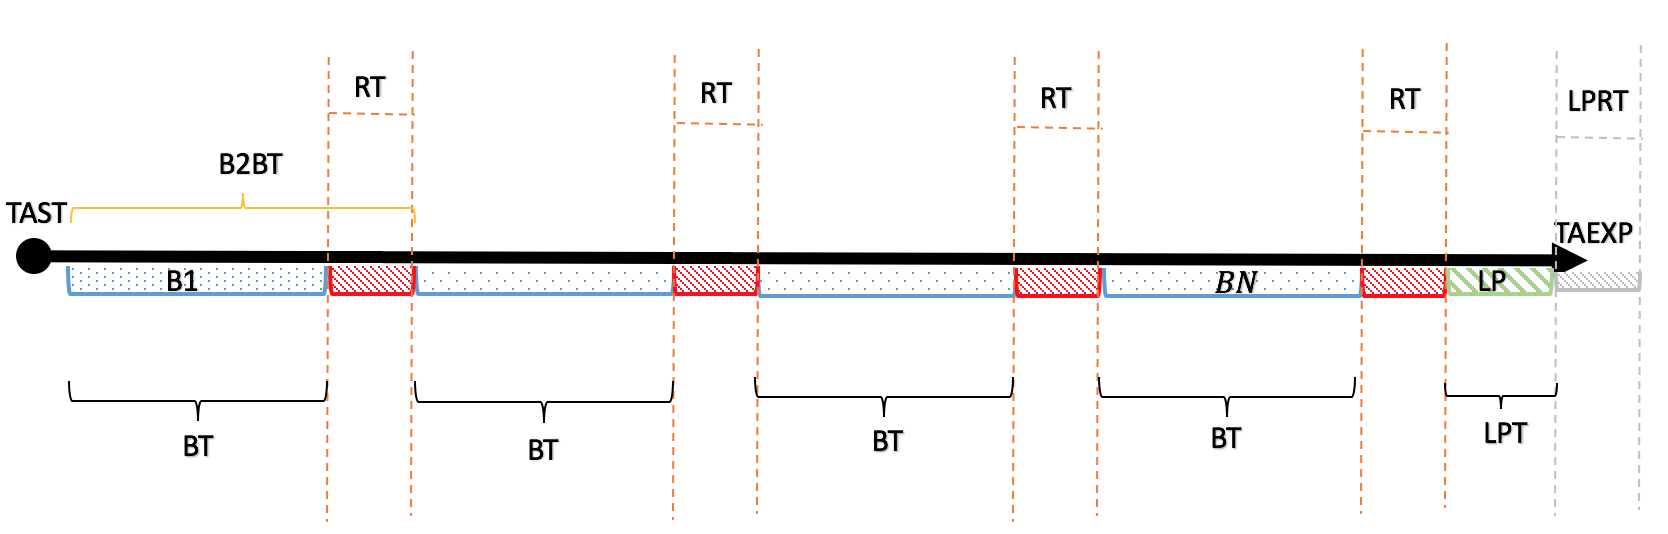
\includegraphics[width=.7\textwidth]{Dis}
	\centering
\end{figure*}



%\anote{EDITED  ABOVE -- ORIGINAL BELOW -- PM}



%\subsection{Data Batching}
%With the absence of central trust, our approach is a receipt-based model. A consumer is required to send a receipt for every data he received, for this, the real-time stream has to be divided into batches.
%
%A data batch is a group of real-time IoT data which is divided into batches in order to has a checking point after each batch. The checking point checks if the batch has been delivered to a consumer. After each batch has been sent, a consumer has to send a receipt to what he received from the previous batch to the smart contract. An acknowledgment will be sent from the smart contract telling the producer that the data which are sent has been delivered then the producer resume sending the next batch. Once a trade agreement expires, a producer stop streaming the data and a consumer has to send a last receipt to settle the trade.
%
%A receipt is a receipt object sent by a consumer to the smart contract. It reports the number of messages delivered by a consumer for batch received.


% While every receipt sent by a consumer needs some gas in order to interact with the smart contract, the less receipts sent means the less gas consumed in smart contract invocation. It is worth to note that specifying the size of the batch is auto-calculated based on a consumer reputation in the marketplace. In other words, a consumer who has high reputation, has large amount of data in a batch which leads to less checking point and therefore less smart contract invocation. 

%
%\mycomment{The batch size is a linear function of a consumer reputation in the marketplace multiplied by a message rate $Rate$} {there is a problem here BS cannot be a rate}.
%	
%	\mycomment{It has to mention that in case of dishonest consumer, a producer will lose at maximum one batch size,}{this is true only if the producer can suspend data delivery and then continue. But i think this is not a viable model.}
%%
%\begin{lstlisting}[basicstyle=\smaller, frame=single]
%ETM = TATI * Rate      
%
%# ETM: Estimated Total Messages in a Trade 
%# TATI: TA Time Interval
% 
%if C_rep =0 Then:
%    A producer has to set the BS manually.
%else:
%    BS = Rate * C_rep
%
%\end{lstlisting}

%It is worth to note that the data stream is a time sensitive which means it will lose its value once it is divided into batches. The time taken between two batches (RT) as shown in figure \ref{Stream} could be a waste time for a consumer to wait for the receipt to be processed. Because of the batch size function is a linear, a consumer with a high reputation score would use most of the contract time to receive data. An honest consumer has batch size larger than dishonest consumer which means less time consumed in receipts processing and therefore more real-time data received. It is a direct proportional between consumer reputation and using the value of the real-time data stream. 

%  While producers generate a real-time data stream which has to be delivered continuously and on the time of its generation or otherwise it will lose its value, some data is tolerant to be interrupted. Because of the needs of the checking point in our model to process batches receipts sent by a consumer, both streams type have to be divided into batches and checking point for receipts will be after each batch. 



% \begin{figure}
%   \caption{Continuous Data Stream}
%   \label{Con}
%   \includegraphics[scale=0.2]{Con}
%   \centering
% \end{figure}

% \begin{figure}
%   \caption{Discontinuous Data Stream (Interrupted tolerance)}
%   \label{Dis}
%   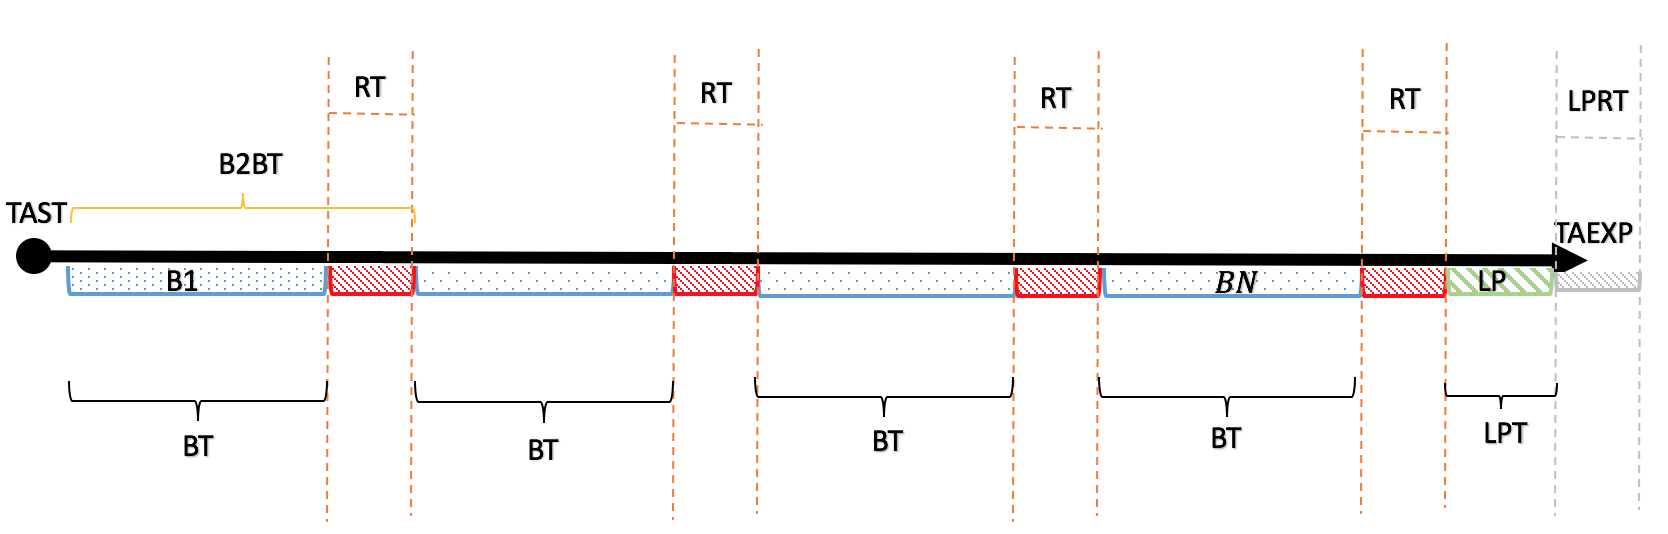
\includegraphics[scale=0.3]{Dis}
%   \centering
% \end{figure}


% % Start the sub figure
% \begin{figure}%
%     \centering
%     \subfloat[Continuous Data Stream]{{\includegraphics[width=9cm]{Con} }}%
%     \qquad
%     \subfloat[Discontinuous Data Stream (Interrupted tolerance)]{{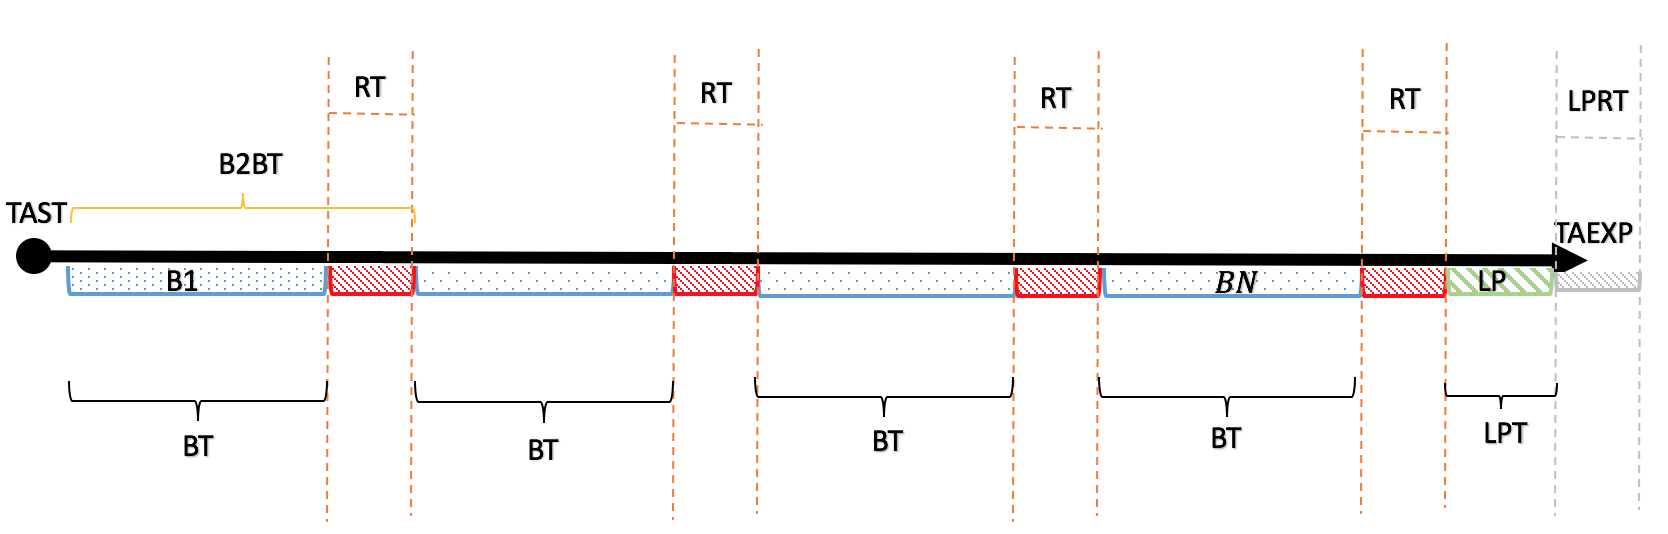
\includegraphics[width=9cm]{Dis} }}%
%     \caption{Data Stream Categories}%
%     \label{ConDisStreams}%
% \end{figure}

\anote{I think this is all we need for this section. much simplified because behind the many equation the storyr is actually very simple, so I commented out the original text--- but please look at the comments.}
%
%\subsection{Last Data Package}
%As agreed in the TA, the data stream will be stopped once the subscription expires. Therefore, if there was a batch has been starting and has not been completed yet, the data provider has to stop streaming the data and the consumer must send a receipt for data portion he received, lets call it (Last Data Package in the trade LP) as shown in figure \ref{Stream}. A processing time for the receipt (LPRT) will be out of TATI which means the smart contract will wait LPRT time to receive the last receipt and then  add it to the total receipts have to make the settlement. It is expected by the smart contract to receive a receipt for the LP within a period of time $LPRT $where $LPRT = RT$.

%\subsection{Participants' loss} \label{ParLoss}
%In the marketplace protocol, and based on the assumption that the data providers are honest while they have no incentives not to sell their data in the marketplace, they have to take a risk when decide to involve in new trades in this marketplace. A producer could reduce his risk and loss by set a minimum reputation for candidate consumers when he pushes an offer in the blockchain, and also can updates the values anytime based on the current market state. 
%
%\mynote{It should mention that a consumer might cheat and does not send a receipt to what he received, and therefore the data owner (producer) will loses the unreported data and the consumer will be rated with low reputation score based on the proposed reputation model of this marketplace.}
%
%A consumer should send a receipt within RT while the producer waiting for the acknowledgment to resume sending the next data batch. If the consumer does not send the receipt or does not report the correct amount of data delivered, the trades stops immediately and a producer can only lose the price of at maximum one full batch as the following where Max and $ P_{Loss} $ are Maximum Data Loss and Producer Loss, respectively:
%\vspace{-0.1 cm}
%\mathleft
%\begin{align}
%\textbf{a) } & Max = BS \nonumber\\
%\textbf{b) }  & 0 <= P_{Loss} <= ( Max \times UP )\nonumber
%% \textbf{c) }  & Max_CLoss = Max_DLoss \times Price \times Price 
%% \nonumber\\
%% \textbf{d) }  &  >= P_CLoss <= Max_CLoss \nonumber
%\end{align}

%\subsection{Settlement Process}
%
%The settlement process is the task of fulfillment the financial contractual obligations of a trade.
%At the end of each trade, the price of the total data delivered (AP) should be taken out from the consumer deposit and transferred to the producer account,  and the rest (if any) will be returned back to a consumer account. When a consumer interact with the smart contract to create a new TA, he deposits tokens for the expected total data price (TP) could to be delivered during the TATI. The expected total data  ETM  and AP are calculated as the following:
%
%\vspace{-0.2 cm}
%\mathleft
%\begin{equation}
%\textbf {$ETM = TATI \times Rate. $}    
%\end{equation}
% 
%\vspace{-0.5 cm}
%% OR \mynote{$ETM = TATI//BS \times Rate$} This exclude the LP ( does not work )
%
%\mathleft
%\begin{equation}
%\textbf {$TP = ETM \times UP $} 
%\end{equation}
%
%\vspace{-0.5 cm}
%
%\mathleft
%\begin{equation}
%\textbf {$AP = UP \times \big(BS \times BN + LP\big)$} 
%\end{equation}
%

%where UP, BS, BN and LP is the price per message unit, the batch size, the batch number and last package data, respectively and $ AP \subset TP$.
%
%Each trade parties in the marketplace costs some tokens for trading. Firstly, everyone in the marketplace has to register in the network by invoking registration method in the smart contract. This cost will be deducted once from their balances and it is called a \textit{registration cost}. \textit{ An offering cost} is the cost deducted from a producer account in order to deploy his offer to the network. He invokes the offer method from the smart contract with his offer details as a transaction payload. \textit{ A set up cost} is deducted for each trade between a producer and a consumer which include all expenses of making an order and creating a new TA from consumer side, and do the data batching and approve the created TA from the producer side. \textit{An Authentication cost} is the cost paid for sending a receipt for every data batch received by a consumer. This cost will be deducted only from consumer balance for sending receipts. This cost will be paid  as receipts cost as the same as the number of batches delivered plus the last package (if any) by a consumer in a trade. Producer and consumer balances will be as follows for trade $T_{i}$ and $offer_{i}$:
%
%\vspace{-0.3 cm}
%
%\mathleft
%\begin{equation}
%\textbf{$P_{balance} -= ( Offering Cost_{i} + Setup Cost_{i} )$} 
%\end{equation}
%
%\vspace{-0.5 cm}
%
%\mathleft
%\begin{equation}
% \textbf{$C_{balance} -= ( C_{cost_{i}} + AP{i} )$}   
%\end{equation}
%
%\vspace{-0.5 cm}
%
%\mathleft
%\begin{equation}
%\textbf{$ C_{cost_{i}} = Setup Cost_{i} + Authentication Cost_{i} $} \label{C_costEq}     
%\end{equation}
%
%
%
%Note: $ Registration Cost$ is excluded because we assumed it was taken once from their balances in their first interaction in the marketplace. 
%
%We will use the following as abbreviation; Gas Used for Registration as GUR, Gas Used for Setup as GUS, Gas Used for Authentication for sending the receipt as GUA, Gas Price by Gwei as GP, Receipt number in a trade as RN, batch number as BN, Last data package LP, Batch sending time as BT, receipt processing time as RT, and time between two batches as B2B.
%
%\vspace{-0.5 cm}
%
%\mathleft
%\begin{equation}
%\textbf{$ Registration Cost = GUR \times GP$ }   
%\end{equation}
%
%\vspace{-0.5 cm}
%
%\mathleft
%\begin{equation}
%\textbf{$ Setup Cost_{i} = GUS_{i} \times GP_{i} $}    
%\end{equation}
%
%\vspace{-0.5 cm}
%
%\mathleft
%\begin{equation}
%\textbf{$ Authentication Cost_{i} =  RN_{i} \times GUA_{i} \times GP_{i} $}    
%\end{equation}
%
%\vspace{-0.5 cm}
%
%\mathleft
%\begin{equation}
%\textbf{$ RN _{i} = BN _{i} + LPN _{i} $}   
%\end{equation}
%
%\vspace{-0.5 cm}
%
%\mathleft
%\begin{equation}
%\textbf{$ LP _{i} = TATI _{i}  \%  B2B _{i} $}   
%\end{equation}
%
%\vspace{-0.5 cm}
%
%\mathleft
%\begin{equation}
%BN _{i} = \frac{TATI _{i}}{B2B _{i}}
%\end{equation}
%
%\vspace{-0.5 cm}
%
%\mathleft
%\begin{equation}
%\textbf{$ B2B _{i} = BT _{i} + RT _{i}$}    
%\end{equation}
%
%\vspace{-0.5 cm}
%
%\mathleft
%\begin{equation}
%BT _{i} = \frac{BS _{i}}{Rate _{i} } 
%\end{equation}
%
%\vspace{-0.5 cm}
%
%\mathleft
%\begin{equation}
%\textbf{$ BS _{i} = C_{Rep} \times Rate $}    
%\end{equation}
%
%\vspace{0.5 cm}
%
%From all the above equations, we could rewrite formula (\ref{C_costEq}) as follows:
%
%% \mathcenter 
%\begin{equation} \label{FCostEq}
%\boldmath C_{cost} = \bigg\{ \big[ \frac{TATI}{C_{Rep}+RT} + LP\big] \times GUA + GUS \bigg\}\times GP
%\end{equation}

%
%Where $C_{cost}$ is a consumer cost in a trade.

\section{System Architecture ans Workflow} \label{Arch}
%%%%%%%%%%%%%%%%%%%%%%%%%%%%%%%%%%%%%%%%%%%%%%%%%

\begin{figure*}
  \caption{System Sequence Diagram}
  \label{SSD}
%   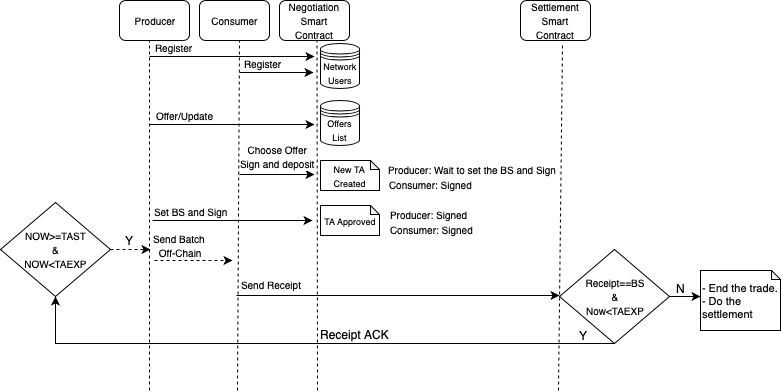
\includegraphics[scale=0.31]{SystemArchWithBackground}
  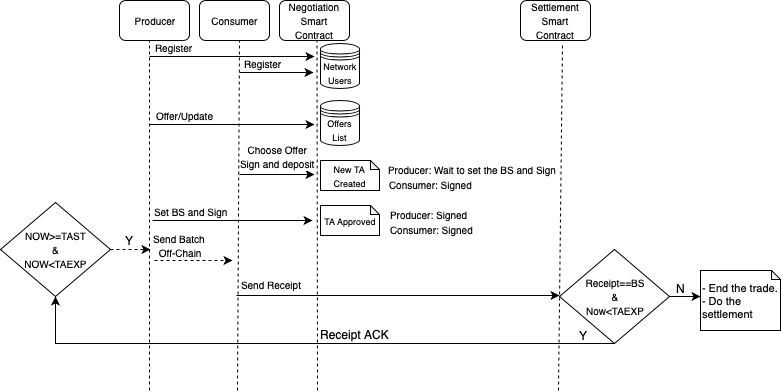
\includegraphics[width=.7\textwidth]{SystemArchWithBackground}
%   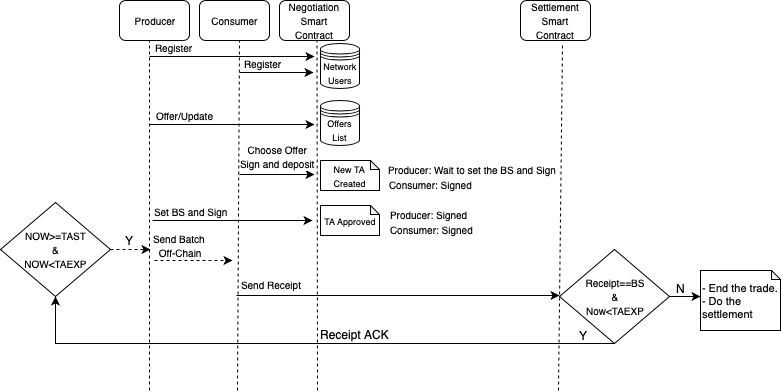
\includegraphics[width=300pt]{SystemArchWithBackground}
  \centering
\end{figure*}

The system is divided into two layers; Data Layer and Blockchain Layer. In data layer, all IoT data will be transferred off chain from data producers to data consumers through brokers in-between, while in the blockchain layer, the negotiation and the the final trade agreement will be created and recorded. The blockchain layer is represented as a set of automated smart contracts written in Solidity (high-level language for writing a smart contract on Ethereum network and executed in Ethereum Virtual Machine EVM in Ethereum network).

As shown in Figure\ref{SSD}, the marketplace starts that each participant must register his address in the blockchain by interacting with the smart contract and calling the register method. A data provider publishes/updates his offers to what data he has. All offers will be stored in the blockchain and visible to anyone. On the other hand, a data consumer checks data providers and their offers, and then when he decides to subscribe data, he has to interact with the smart contract with his offer’s choice and the time interval who would like the subscription start and end. A new TA is created and signed by consumer by his private key in the blockchain and has been deployed. Next, a data provider checks this consumer’s reputation in the marketplace and then set the data batch size if it is zero or it would be calculated automatically, add it to the TA and then deployed it to the blockchain with his signature. Now, we have a new TA signed by both trade’s parties and visible to anyone and can not be amended. 

The data provider at the start time of the subscription starts sending the data batches as agreed in the TA. When a first batch has been sent, a consumer should send a receipt to the smart contract reporting what he received. A smart contract will check if the data received is equal to the batch size set in the agreement, meanwhile, the provider is paused and waiting for the acknowledgment to be triggered. If the data delivered was not equal the data batch, the smart contract will trigger an event that the trade is going to fail and therefore, the reputation and settlement contract ends the the trade immediately and release the tokens to the producer as mush as reported in the receipt and return back the rest to the consumer balance. Eventually, a reputation score is updated and eventually the trade is labeled failed. 
% %%%%%%%%%%%%%%%%%%%%%%%%%%%%%%%%%%%%%%%%%%%%%%%%%

\section{Implementation and evaluation} \label{sec:evaluation}

The decentralized brokered IoT data marketplace model has implemented the trade management and the settlement service as set of smart contracts in the blockchain written by the high-level language \textit{Solidity} in Ethereum platform. 

For experimentation and evaluation purposes, we have written a smart contract in Solidity – Ethereum’s scripting language and then deployed it in a private Ethereum test network. We used Ethereum web browser based IDE Remix \cite{25} to write, deploy and connect to the private chain through Remote Producer Call (RPC) protocol. We have used the fake accounts with their balances provided by Remix (each with 100 ether) as a trades’ participants e.g. producer and consumer. 

Each account has to interact with the smart contract in order to register in the network by providing a name and the role type to act in the network, e.g. producer or consumer. Then, a producer consumes gas to interact with the smart contact to deploy his offer to the network, and on the other hand a consumer interacts to get an offer. Another gas consumption for the consumer is in interacting with the smart contract to make an order based on provided offers, initiate a new TA and deposit the full amount of the trade based on the estimated data amount might be delivered in a trade ETM. In this stage, a batch size has been set based on the consumer reputation and eventually sign the current TA with this candidate consumer. 

Based on the protocol proposed, the consumer has to send a receipt for every batch received. He costs an authentication fees (BN + LPN) times where BN and LPN is the total number of batches received in a trade and the last data package (1 if any, 0 otherwise), respectively. Table \ref{GasTable} shows the gas consumed by each producer and consumer for a trade in the marketplace. We have measured the gas consumption using Remix debugger which provide a consumed gas for every transaction done. Also, it can be calculated by monitoring the balances of participants and check the differences before and after invoking the smart contract method. Table \ref{GasTable} shows the cost categories whose either producer or consumer or both have to spend.

\begin{table}[h]
\caption{shows transactions cost in each cost category (in Gas)}
\label{GasTable}
\begin{center}
% \begin{adjustbox}{max height=4 \textheight, width=0.55\textwidth }
\begin{tabular}{|m{15mm}||m{20mm}||m{15mm}||m{15mm}|}
\hline
\textbf{\makecell{Cost\\Category}}&
\centering\textbf{Operation}&
\textbf{\makecell{Producer\\Gas\\Consumption}} & 
\textbf{\makecell{Consumer\\Gas\\Consumption}} \\
\hline
\centering\makecell{Registration \\Cost} & \makecell{- Register \\in\\ the network} & 204739 gas & 199093 gas 
  \\
\hline
\makecell{Offering \\Cost} & - Deploy an offer & 491862 gas & - \\
\hline
\multirow{2}{*}\centering{\makecell{Setup\\Cost}} & \makecell{- Make an order \\and create \\ a new TA} & - & 620865 gas \\

& \makecell{- Set Batch size \\and sign off \\ the TA} & 82063 gas & - \\ 
\hline
\makecell{Authentication\\Cost} & - Send a receipt & - &  144367 gas \\

\hline
\end{tabular}
% \end{adjustbox}
\end{center}
\end{table}
% 

The settlement is done by the settlement smart contract when the trade ends. 
The consumer honesty defines the batch size of the data in a trade due to the proposed protocol that the batch is a function of a consumer reputation in the marketplace. If a consumer reputation is high, a batch size will be large and a he can receive more data in one batch. Similarly, a consumer who has a low reputation receives a less data in the batch. The increase in a number of batches received means that a consumer will cost more gas to interact with the smart contract to send receipts. If we assume that a producer has no incentive not to send the data as agreed in the TA, and with a guarantee the quality of service, a trade would be failed if a consumer was not send a receipt or was not honest in reporting the exact number of data he received. It is crucial for a marketplace sustainability to have an honest consumer in order to have successful trades, and also for the consumer financial affairs to be avoided from many smart contract invocations and therefore extra cost (authentication cost).

In our evaluation, we focus on the association between consumers’ honesty (reputation) and the cost they have to spend to reach to a successful trade. An honest consumer who has high reputation spends less than a consumer who has low reputation. When a consumer is an honest, he shows his willing to behave well in the marketplace which significantly reflect on the batch size of that trade who involve in. While the batch size is directly proportional to consumer honesty, this would be a motivation for a consumer to have high reputation in order to reduce his cost.

Because a gas price determines the average time of the transactions in the blockchain to be processed by miners, a consumer has the potential to increase the gas price in order to process his transaction faster and therefore he will have more time to receive more batches. 

It has to notice that the transaction of sending receipts to the smart contract has to be processed in the period of time, so a consumer may increase the gas price of his transactions to give his transaction the priority to be picked by miners. Miners who will validate the transactions usually follow the strategy of picking the transactions’ heights gas price to be included in the next block in order for high rewards. Because of the transactions fees goes to the miners as rewards for their verification, a consumer may set gas price high enough to encourage miners to select his transaction to be involved in their next block. The increase in the gas price may contribute in decreasing the receipt processing time RT and therefore more time to receive more batches within TATI

A minimum and the maximum gas price in the network could be known and limit in ETH Gas Station \cite{13}.  ETH Gas Station is a tool to understand the conditions of the current gas market and current policies of network miners. 

Based on the current condition of the network at the moment of writing, the recommended gas prices from \cite{13} has been shown in table \ref{GasPriceTable} . It shows the maximum time taken by miners to confirm the transaction for each GP. In addition, \cite{13} provides the median time of transaction confirmation for each gas price.
\begin{table}[h]
\caption{Gas Prices and Speeds}
\label{GasPriceTable}
\begin{center}
\begin{tabular}{|c||c||c|}
\hline
\textbf{\makecell{Gas Price\\ (Gwei)}} &\textbf{Speed} & \textbf{Median Speed}\\

\hline
1.6  & SafeLow (\textless30m) & 2.5m \\

\hline
4.2  & Standard (\textless5m) & 1.5m \\
\hline
7.2  & Fast (\textless2m) & 0.8m \\

\hline
\end{tabular}
\end{center}
\end{table}

For the purpose of evaluating that the cost is inversely proportional to the reputation, we have fixed the parameters TATI with 1 day (24 hours), GUA and GUS as mentioned earlier in table \ref{GasTable} and use the three different GP for different consumer reputations to calculate the $C_{cost}$ (Eq.\ref{FCostEq}) in table \ref{CostTable} 


\begin{table}[h]
% \begin{center}
\caption{Shows the cost in USD for consumer reputations for 1 day trade with three GP values, Rate 100 msg/sec. (1 Eth $\approx$ 202.70 USD)}
\label{CostTable}
% \begin{center}
\begin{adjustbox}{width=0.48\textwidth}
\begin{tabular}{|c||c||c||c|}
\hline
\textbf{Consumer} & \multicolumn{3}{c}{\textbf{Consumer Cost (Setup + Authentication) in USD}}\\ 
\textbf{Reputation}  & \textbf{ GP= 1.6 Gwei} & \textbf{GP = 4.2 Gwei} & \textbf{GP= 7.2 Gwei} \\ 
\hline
$0.1$ & $ 25.48 \$ $ & $ 106.72 \$ $ & $ 314.98 \$ $ \\
\hline
$0.2$ & $ 24.04 \$ $ & $ 97.19 \$ $ & $ 268.82 \$ $ \\
\hline
$0.3$ & $ 22.68 \$ $ & $ 89.02 \$ $ & $ 234.50 \$ $ \\
\hline
$0.4$ & $ 21.54 \$ $ & $ 82.33 \$ $ & $ 207.98 \$ $ \\
\hline
$0.5$ & $ 20.43 \$ $ & $ 76.50 \$ $ & $ 186.87 \$ $ \\
\hline
$0.6$ & $ 19.51 \$ $ & $ 71.32 \$ $ & $ 169.46 \$ $ \\
\hline
$0.7$ & $ 18.64 \$ $ & $ 66.90 \$ $ & $ 155.39 \$ $ \\
\hline
$0.8$ & $ 17.84 \$ $ & $ 63.12 \$ $ & $ 143.36 \$ $ \\
\hline
$0.9$ & $ 17.06 \$ $ & $ 59.52 \$ $ & $ 133.03 \$ $ \\
\hline
$1.0$ & $ 16.43 \$ $ & $ 56.54 \$ $ & $ 124.12 \$ $ \\
\hline 

\end{tabular}
\end{adjustbox}
% \end{center}
\end{table}

\begin{figure}%
    \centering
    \subfloat[Number of Receipts]{{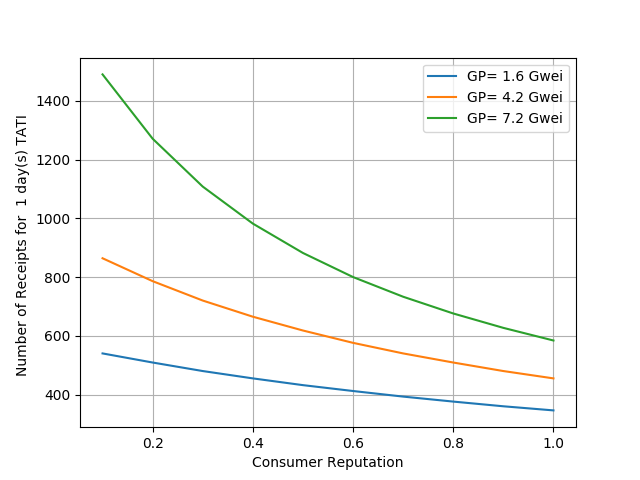
\includegraphics[width=6cm]{Receipts} }}%
    \qquad
    \subfloat[Cost in USD]{{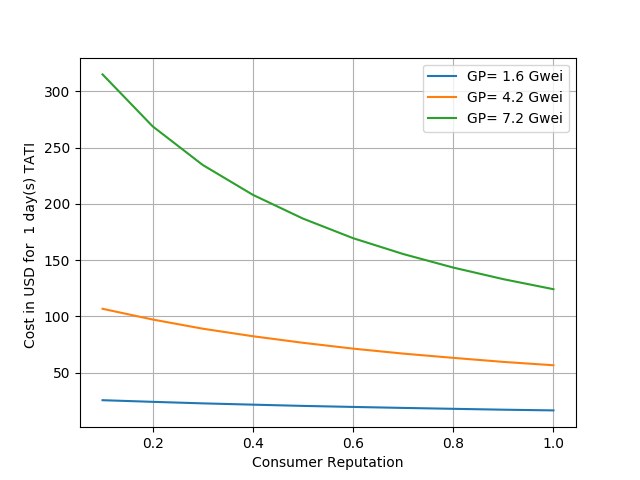
\includegraphics[width=6cm]{cost} }}%
    \qquad
     \subfloat[Data Percentage Received]{{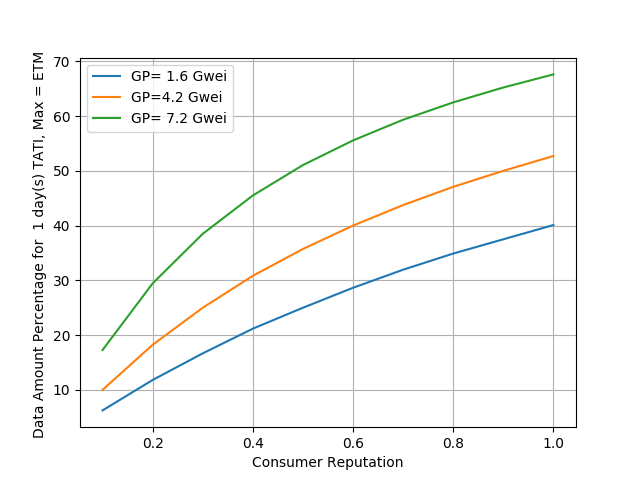
\includegraphics[width=6cm]{Data} }}%
    \caption{The cost, the number of receipts and the percentage of the data received for three different gas prices}%
    \label{2FigEvaluation}%
\end{figure}

 In figure \ref{2FigEvaluation} (a), the smart contract invocations represented by number of receipts have been increasing for lower consumer reputation and gradually decreased for high reputation. The cost of these invocations have been represented in figure \ref{2FigEvaluation} (b).
%  Note: The cost represented in the figure \ref{2FigEvaluation} is $C_{cost}$.
 
% It is worth to mention that in terms of data producer, he checks the consumer reputation in order to approve a consumer request. The increase in consumer cost by increasing the gas price is not necessary for a producer to accept consumer request and initiate a new trade. While it could be a vital factor for a consumer to increase his reputation faster if and only if the current trade ends successfully. It depends on a producer decision to take this risk and get involve in this trade.

It is worth to mention that in terms of consumer cost as shown in table \ref{CostTable}, many consumers would prefer to pay the lowest gas possible  because the difference between the cost for a 0.1 consumer reputation and 1.0 is only 9.05 \$ and it is not very high value for one day trade. But In terms of data amount received, figure \ref{2FigEvaluation} (c) has shown that the former has received only about 6.25 \% from the estimated data delivered while the latter has received about 40.10 \% and in real-time data trades, the amount of trade received is the core factor for the consumer, otherwise, the data will lose its value if it is received after long time of its generation. 


% \section{MATH}

% Before you begin to format your paper, first write and save the content as a separate text file. Keep your text and graphic files separate until after the text has been formatted and styled. Do not use hard tabs, and limit use of hard returns to only one return at the end of a paragraph. Do not add any kind of pagination anywhere in the paper. Do not number text heads-the template will do that for you.

% Finally, complete content and organizational editing before formatting. Please take note of the following items when proofreading spelling and grammar:

% \subsection{Abbreviations and Acronyms} Define abbreviations and acronyms the first time they are used in the text, even after they have been defined in the abstract. Abbreviations such as IEEE, SI, MKS, CGS, sc, dc, and rms do not have to be defined. Do not use abbreviations in the title or heads unless they are unavoidable.

% \subsection{Units}

% \begin{itemize}

% \item Use either SI (MKS) or CGS as primary units. (SI units are encouraged.) English units may be used as secondary units (in parentheses). An exception would be the use of English units as identifiers in trade, such as Ò3.5-inch disk driveÓ.
% \item Avoid combining SI and CGS units, such as current in amperes and magnetic field in oersteds. This often leads to confusion because equations do not balance dimensionally. If you must use mixed units, clearly state the units for each quantity that you use in an equation.
% \item Do not mix complete spellings and abbreviations of units: ÒWb/m2Ó or Òwebers per square meterÓ, not Òwebers/m2Ó.  Spell out units when they appear in text: Ò. . . a few henriesÓ, not Ò. . . a few HÓ.
% \item Use a zero before decimal points: Ò0.25Ó, not Ò.25Ó. Use Òcm3Ó, not ÒccÓ. (bullet list)

% \end{itemize}


% \subsection{Equations}

% The equations are an exception to the prescribed specifications of this template. You will need to determine whether or not your equation should be typed using either the Times New Roman or the Symbol font (please no other font). To create multileveled equations, it may be necessary to treat the equation as a graphic and insert it into the text after your paper is styled. Number equations consecutively. Equation numbers, within parentheses, are to position flush right, as in (1), using a right tab stop. To make your equations more compact, you may use the solidus ( / ), the exp function, or appropriate exponents. Italicize Roman symbols for quantities and variables, but not Greek symbols. Use a long dash rather than a hyphen for a minus sign. Punctuate equations with commas or periods when they are part of a sentence, as in

% $$
% \alpha + \beta = \chi \eqno{(1)}
% $$

% Note that the equation is centered using a center tab stop. Be sure that the symbols in your equation have been defined before or immediately following the equation. Use Ò(1)Ó, not ÒEq. (1)Ó or Òequation (1)Ó, except at the beginning of a sentence: ÒEquation (1) is . . .Ó

% \subsection{Some Common Mistakes}
% \begin{itemize}


% \item The word ÒdataÓ is plural, not singular.
% \item The subscript for the permeability of vacuum ?0, and other common scientific constants, is zero with subscript formatting, not a lowercase letter ÒoÓ.
% \item In American English, commas, semi-/colons, periods, question and exclamation marks are located within quotation marks only when a complete thought or name is cited, such as a title or full quotation. When quotation marks are used, instead of a bold or italic typeface, to highlight a word or phrase, punctuation should appear outside of the quotation marks. A parenthetical phrase or statement at the end of a sentence is punctuated outside of the closing parenthesis (like this). (A parenthetical sentence is punctuated within the parentheses.)
% \item A graph within a graph is an ÒinsetÓ, not an ÒinsertÓ. The word alternatively is preferred to the word ÒalternatelyÓ (unless you really mean something that alternates).
% \item Do not use the word ÒessentiallyÓ to mean ÒapproximatelyÓ or ÒeffectivelyÓ.
% \item In your paper title, if the words Òthat usesÓ can accurately replace the word ÒusingÓ, capitalize the ÒuÓ; if not, keep using lower-cased.
% \item Be aware of the different meanings of the homophones ÒaffectÓ and ÒeffectÓ, ÒcomplementÓ and ÒcomplimentÓ, ÒdiscreetÓ and ÒdiscreteÓ, ÒprincipalÓ and ÒprincipleÓ.
% \item Do not confuse ÒimplyÓ and ÒinferÓ.
% \item The prefix ÒnonÓ is not a word; it should be joined to the word it modifies, usually without a hyphen.
% \item There is no period after the ÒetÓ in the Latin abbreviation Òet al.Ó.
% \item The abbreviation Òi.e.Ó means Òthat isÓ, and the abbreviation Òe.g.Ó means Òfor exampleÓ.

% \end{itemize}


% \section{USING THE TEMPLATE}

% Use this sample document as your LaTeX source file to create your document. Save this file as {\bf root.tex}. You have to make sure to use the cls file that came with this distribution. If you use a different style file, you cannot expect to get required margins. Note also that when you are creating your out PDF file, the source file is only part of the equation. {\it Your \TeX\ $\rightarrow$ PDF filter determines the output file size. Even if you make all the specifications to output a letter file in the source - if you filter is set to produce A4, you will only get A4 output. }

% It is impossible to account for all possible situation, one would encounter using \TeX. If you are using multiple \TeX\ files you must make sure that the ``MAIN`` source file is called root.tex - this is particularly important if your conference is using PaperPlaza's built in \TeX\ to PDF conversion tool.

% \subsection{Headings, etc}

% Text heads organize the topics on a relational, hierarchical basis. For example, the paper title is the primary text head because all subsequent material relates and elaborates on this one topic. If there are two or more sub-topics, the next level head (uppercase Roman numerals) should be used and, conversely, if there are not at least two sub-topics, then no subheads should be introduced. Styles named ÒHeading 1Ó, ÒHeading 2Ó, ÒHeading 3Ó, and ÒHeading 4Ó are prescribed.

% \subsection{Figures and Tables}

% Positioning Figures and Tables: Place figures and tables at the top and bottom of columns. Avoid placing them in the middle of columns. Large figures and tables may span across both columns. Figure captions should be below the figures; table heads should appear above the tables. Insert figures and tables after they are cited in the text. Use the abbreviation ÒFig. 1Ó, even at the beginning of a sentence.



%   \begin{figure}[thpb]
%       \centering
%       \framebox{\parbox{3in}{We suggest that you use a text box to insert a graphic (which is ideally a 300 dpi TIFF or EPS file, with all fonts embedded) because, in an document, this method is somewhat more stable than directly inserting a picture.
% }}
%       %\includegraphics[scale=1.0]{figurefile}
%       \caption{Inductance of oscillation winding on amorphous
%       magnetic core versus DC bias magnetic field}
%       \label{figurelabel}
%   \end{figure}
   

% Figure Labels: Use 8 point Times New Roman for Figure labels. Use words rather than symbols or abbreviations when writing Figure axis labels to avoid confusing the reader. As an example, write the quantity ÒMagnetizationÓ, or ÒMagnetization, MÓ, not just ÒMÓ. If including units in the label, present them within parentheses. Do not label axes only with units. In the example, write ÒMagnetization (A/m)Ó or ÒMagnetization {A[m(1)]}Ó, not just ÒA/mÓ. Do not label axes with a ratio of quantities and units. For example, write ÒTemperature (K)Ó, not ÒTemperature/K.Ó

\section{CONCLUSIONS} \label{conclusion}

This paper introduces a decentralized marketplace for trading brokered IoT data, and leverage the model with blockchain technology as distributed, immutable and public records. It is structured into two entities: (1) the standard IoT brokered data protocol and on the top and (2) the settlement system provider (as an automated smart contracts on the blockchain network). Every trade has a trade contract signed by both participants and then kept in the blockchain. A TA is a tuple of all trade details between a producer and a consumer.

While the approach in this model is a receipt-based, the real-time data stream is divided into batches which is a linear function of a consumer honesty in the marketplace. A consumer honesty is measured by the consumer commitment to send a receipt for every data delivered in each batch.
As shown, the expenses of having a trade on the blockchain has been categorized into four; registration fees, offering fees, setup fees and the authentication fees. 
There is a inverse proportion between a consumer reputation and an authentication cost. The evaluation shows that the consumer with high reputation get a small number of batches and therefore less number of smart contract interaction to send receipts. A consumer with low reputation get high number of batches and therefore more gas consumed to interact with the smart contract to send the receipts. 

% \addtolength{\textheight}{-12cm}   % This command serves to balance the column lengths
%                                   % on the last page of the document manually. It shortens
%                                   % the textheight of the last page by a suitable amount.
%                                   % This command does not take effect until the next page
%                                   % so it should come on the page before the last. Make
%                                   % sure that you do not shorten the textheight too much.

% %%%%%%%%%%%%%%%%%%%%%%%%%%%%%%%%%%%%%%%%%%%%%%%%%%%%%%%%%%%%%%%%%%%%%%%%%%%%%%%%



% %%%%%%%%%%%%%%%%%%%%%%%%%%%%%%%%%%%%%%%%%%%%%%%%%%%%%%%%%%%%%%%%%%%%%%%%%%%%%%%%



% %%%%%%%%%%%%%%%%%%%%%%%%%%%%%%%%%%%%%%%%%%%%%%%%%%%%%%%%%%%%%%%%%%%%%%%%%%%%%%%%
% % \section*{APPENDIX}

% % Appendixes should appear before the acknowledgment.

\section*{ACKNOWLEDGMENT}

This research has been funded by Umm AlQura University, Makkah, The Kingdom of Saudi Arabia.



%%%%%%%%%%%%%%%%%%%%%%%%%%%%%%%%%%%%%%%%%%%%%%%%%%%%%%%%%%%%%%%%%%%%%%%%%%%%%%%%
\bibliographystyle{unsrt}
\bibliography{sample,iot-conf}

\end{document}
